\documentclass[11pt,fleqn]{article}

\setlength {\topmargin} {-.15in}
\setlength {\textheight} {8.6in}

\usepackage{amsmath}
\usepackage{amssymb}
\usepackage{color}
\usepackage{tikz}
\usetikzlibrary{automata,positioning,arrows}
\usepackage{diagbox}



\newcommand{\be}{\begin{enumerate}}
\newcommand{\ee}{\end{enumerate}}

\begin{document}
\begin{center}
	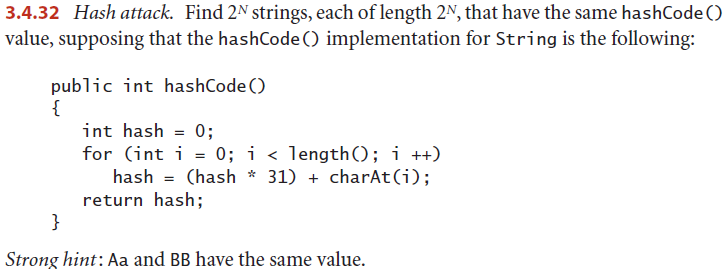
\includegraphics[scale=.85]{3.4.32.png}
\end{center}
	
\textbf{Solution:}\\
Lets say the two strings are AaAa AND BBBB. This problem is quite simple as its just the overall ASCII value you get from a string. For example, BBAa has the same ASCII as AaBB. So you can re-arrange your strings in any way aslong as its the same number of each character in the string.


\end{document}
